\documentclass[11pt,a4paper]{article}

% ==============================================================================
% PACKAGES & SYSTEM CONFIGURATION
% ==============================================================================
\usepackage[utf8]{inputenc}
\usepackage[margin=0.9in]{geometry}
\usepackage{graphicx}
\usepackage{hyperref}
\usepackage{amsmath,amssymb}
\usepackage{booktabs}
\usepackage{tabularx}
\usepackage{caption}
\usepackage{subcaption}
\usepackage{float}
\usepackage{enumitem}
\usepackage{xcolor}
\usepackage{fancyhdr}
\usepackage{lastpage}
\usepackage{titlesec}
\usepackage{listings}
\usepackage[many]{tcolorbox}
\usepackage{tikz}
\usetikzlibrary{arrows.meta, positioning, shapes.geometric, fit, backgrounds, calc}

% ==============================================================================
% MODERN COLOR PALETTE
% ==============================================================================
\definecolor{primary}{HTML}{0A2540}    % Deep Navy Blue
\definecolor{secondary}{HTML}{1D3557}  % Slate Navy
\definecolor{accent}{HTML}{0066CC}     % High-visibility Azure Blue
\definecolor{darkgray}{HTML}{2B2D42}   % Body Charcoal
\definecolor{lightbg}{HTML}{F8FAFC}    % Clean Card Background
\definecolor{bordercolor}{HTML}{E2E8F0}% Elegant Border
\definecolor{codebg}{HTML}{F1F5F9}     % Soft Code Gray
\definecolor{boxbg}{HTML}{EBF3F9}      % Subtle Blue Tint
\definecolor{successgreen}{HTML}{2A9D8F}% Success

% ==============================================================================
% HYPERREF SETUP
% ==============================================================================
\hypersetup{
    colorlinks=true,
    linkcolor=accent,
    citecolor=accent,
    urlcolor=accent,
    pdfauthor={Sunil Kumar (12342170)},
    pdftitle={Lab 8: OpenTelemetry Observability Implementation - Village Pond Planning System},
    pdfsubject={OpenTelemetry Distributed Tracing, Metrics, and Log Correlation Report},
    pdfkeywords={OpenTelemetry, Jaeger, Prometheus, Distributed Tracing, Observability, FastAPI, Remote Server}
}

% ==============================================================================
% TYPOGRAPHY & SECTION HEADERS
% ==============================================================================
\titleformat{\section}
  {\Large\bfseries\color{primary}}
  {\thesection}{1em}{}
  [{\color{accent}\titlerule[1.5pt]}]

\titleformat{\subsection}
  {\large\bfseries\color{secondary}}
  {\thesubsection}{1em}{}

\titleformat{\subsubsection}
  {\normalsize\bfseries\color{darkgray}}
  {\thesubsubsection}{1em}{}

% ==============================================================================
% HEADER & FOOTER CONFIGURATION
% ==============================================================================
\pagestyle{fancy}
\fancyhf{}
\fancyhead[L]{\small\color{gray}\textbf{CSD Lab 8:} OpenTelemetry Observability Implementation}
\fancyhead[R]{\small\color{gray}Distributed Systems}
\fancyfoot[L]{\small\color{gray}Sunil Kumar (Roll No: 12342170)}
\fancyfoot[R]{\small\color{gray}Page \thepage\ of \pageref{LastPage}}
\renewcommand{\headrulewidth}{0.4pt}
\renewcommand{\footrulewidth}{0.4pt}

% ==============================================================================
% TCOLORBOX CALLOUT STYLES
% ==============================================================================
\newtcolorbox{infobox}[1][]{
  enhanced,
  colback=lightbg,
  colframe=accent,
  left=12pt,
  right=12pt,
  top=10pt,
  bottom=10pt,
  boxrule=1pt,
  arc=4pt,
  title=\textbf{#1},
  coltitle=white,
  colbacktitle=accent,
  fonttitle=\bfseries
}

\newtcolorbox{summarybox}{
  enhanced,
  colback=codebg,
  colframe=bordercolor,
  left=10pt,
  right=10pt,
  top=8pt,
  bottom=8pt,
  boxrule=0.8pt,
  arc=3pt
}

% ==============================================================================
% LISTINGS CODE CONFIGURATION
% ==============================================================================
\lstset{
  backgroundcolor=\color{codebg},
  basicstyle=\ttfamily\footnotesize\color{darkgray},
  breakatwhitespace=false,
  breaklines=true,
  captionpos=b,
  commentstyle=\color{gray},
  keepspaces=true,
  keywordstyle=\color{accent}\bfseries,
  numberstyle=\tiny\color{gray},
  numbers=none,
  showspaces=false,
  showstringspaces=false,
  showtabs=false,
  stringstyle=\color{successgreen},
  tabsize=2,
  frame=single,
  rulecolor=\color{bordercolor}
}

% ==============================================================================
% DOCUMENT CONTENT STARTS HERE
% ==============================================================================
\begin{document}

% ------------------------------------------------------------------------------
% SECTION 01: TITLE PAGE (CLEAN, ONLY NAME, ROLL, SSH COMMAND & MAIN URL)
% ------------------------------------------------------------------------------
\begin{titlepage}
    \centering
    \vspace*{1.2cm}
    
    \begin{tcolorbox}[enhanced, colback=lightbg, colframe=primary, boxrule=1.5pt, arc=6pt, width=0.96\textwidth]
        \centering\vspace{0.4cm}
        {\LARGE\textbf{\color{primary}LAB 8 REPORT}}\\[0.35cm]
        {\huge\textbf{\color{accent}OpenTelemetry Observability Implementation}}\\[0.45cm]
        {\Large\textbf{Distributed Tracing, Real-Time Metrics, and Trace-Log Correlation in AI-Based Village Pond Planning System}}\\[0.4cm]
    \end{tcolorbox}
    
    \vspace{2.0cm}
    
    \begin{minipage}[t]{0.85\textwidth}
        \centering
        {\LARGE\textbf{Sunil Kumar}}\\[0.3cm]
        {\Large\textbf{Roll Number:}\ \texttt{12342170}}\\[0.2cm]
    \end{minipage}

    \vspace{2.2cm}
    
    \begin{tcolorbox}[enhanced, colback=codebg, colframe=accent, boxrule=1.2pt, arc=5pt, width=0.92\textwidth]
        \centering\vspace{0.2cm}
        \textbf{\color{primary}Project Repository (GitHub):}\\[0.1cm]
        \href{https://github.com/sunilkumar2170/village-pond-planning-opentelemetry}{\texttt{https://github.com/sunilkumar2170/village-pond-planning-opentelemetry}}\\[0.4cm]
        
        \textbf{\color{primary}Remote Server SSH Access (Port 6213):}\\[0.15cm]
        \colorbox{lightbg}{\large\textbf{\texttt{ssh -p 6213 student@10.1.75.53}}}\\[0.4cm]
        
        \textbf{\color{primary}Live Application Endpoint:}\\[0.1cm]
        \url{http://10.1.75.53:3213/}\\[0.2cm]
    \end{tcolorbox}
    
    \vfill
    {\small\color{gray}Evaluation \& Verification Report}
\end{titlepage}

\newpage
\tableofcontents
\newpage

% ------------------------------------------------------------------------------
% SECTION 02: ABSTRACT AND OBJECTIVES
% ------------------------------------------------------------------------------
\section{Abstract and Objectives}

\subsection{Abstract}
In distributed architectures, microservices, and compute-intensive geospatial backends, triaging intermittent latency spikes and understanding service dependencies cannot rely solely on unstructured console print statements. OpenTelemetry (OTel) is the industry-standard, vendor-agnostic observability framework governed by the Cloud Native Computing Foundation (CNCF), providing uniform telemetry specifications across Traces, Metrics, and Logs. 

This report documents the design, instrumentation, and empirical verification of OpenTelemetry within the \textbf{AI-Based Village Pond Planning and Catchment Estimation System} (Assignment 1). The application backend was instrumented with the OpenTelemetry Python SDK to stream distributed traces over OTLP gRPC to a standalone Jaeger collector, expose Prometheus-format system and business metrics on a standardized HTTP endpoint, and achieve deterministic trace-log correlation by injecting 32-character hexadecimal \texttt{trace\_id} and 16-character \texttt{span\_id} tokens into every log record. Experimental analysis successfully pinpointed external meteorological network latency as consuming $56.2\%$ of the total pipeline runtime, demonstrating how observability transforms opaque backend execution into actionable engineering intelligence.

\subsection{Objectives}
The core objectives accomplished in this implementation include:
\begin{enumerate}[leftmargin=*]
    \item \textbf{Complete Three-Pillar Observability}: Implement distributed tracing, Prometheus-compatible metrics exposition, and correlated logging within an existing production-grade geospatial backend.
    \item \textbf{Fine-Grained Domain Tracing}: Break down monolithic request execution into a hierarchical waterfall tree comprising a root HTTP span and seven (7) sequential domain child spans corresponding to spatial parsing, Delaunay grid generation, local elevation minima selection, D8 flow routing, and SCS-CN volumetric runoff calculations.
    \item \textbf{Rich Semantic Attribute Annotation}: Contextualize execution spans with domain-specific metadata (geographic coordinates, terrain elevation, delineated catchment area in hectares, and expected harvestable water volume in cubic meters).
    \item \textbf{Production Verification \& Remote Deployment}: Run the instrumented services locally and deploy to the remote laboratory evaluation server (\texttt{10.1.75.53} via SSH port \texttt{6213}), executing analysis payloads and capturing quantitative verification evidence through Jaeger UI, Prometheus endpoints, and a custom in-memory telemetry dashboard.
\end{enumerate}

% ------------------------------------------------------------------------------
% SECTION 03: APPLICATION OVERVIEW
% ------------------------------------------------------------------------------
\section{Application Overview}

The \textbf{Village Pond Planning System} is a geospatial civil-engineering platform developed to assist rural planners in determining the hydrologically optimal location and storage capacity for rainwater harvesting ponds.

\subsection{End-to-End Processing Workflow}
The application exposes an asynchronous REST API endpoint (\texttt{POST /analyzeContour}) that accepts either a 1-meter elevation contour dataset in KML format or an interactive freehand boundary polygon. The internal processing pipeline executes six discrete algorithmic phases:

\begin{figure}[H]
    \centering
    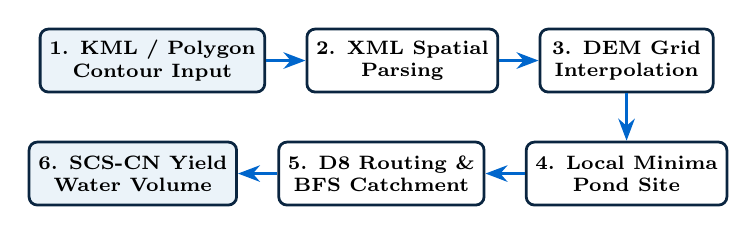
\begin{tikzpicture}[
        node distance=0.4cm and 0.5cm,
        box/.style={rectangle, draw=primary, fill=white, rounded corners=3pt, line width=1pt, minimum width=2.2cm, minimum height=0.8cm, align=center, font=\scriptsize\bfseries},
        arrow/.style={->, >=Stealth, draw=accent, line width=1.1pt}
    ]
        \node[box, fill=boxbg] (input) {1. KML / Polygon\\Contour Input};
        \node[box, right=of input] (kml) {2. XML Spatial\\Parsing};
        \node[box, right=of kml] (grid) {3. DEM Grid\\Interpolation};
        \node[box, below=0.6cm of grid] (pond) {4. Local Minima\\Pond Site};
        \node[box, left=of pond] (d8) {5. D8 Routing \&\\BFS Catchment};
        \node[box, left=of d8, fill=boxbg] (scs) {6. SCS-CN Yield\\Water Volume};

        \draw[arrow] (input) -- (kml);
        \draw[arrow] (kml) -- (grid);
        \draw[arrow] (grid) -- (pond);
        \draw[arrow] (pond) -- (d8);
        \draw[arrow] (d8) -- (scs);
    \end{tikzpicture}
    \caption{Functional computational pipeline of the Village Pond Planning System.}
    \label{fig:app_workflow}
\end{figure}

\begin{enumerate}[leftmargin=*]
    \item \textbf{KML Spatial Parsing (\texttt{kml.parse\_contours})}: Parses XML contour geometry using \texttt{fastkml} and extracts 3D coordinate vertices $(x_i, y_i, z_i)$.
    \item \textbf{Boundary Containment Filtering (\texttt{terrain.boundary\_filtering})}: Evaluates vertices against user-defined region boundaries using Shapely's spatial predicates (\texttt{prep(boundary\_polygon)}).
    \item \textbf{Digital Elevation Model (DEM) Grid Interpolation (\texttt{terrain.build\_elevation\_grid})}: Uses Delaunay triangulation and cubic spline interpolation via \texttt{scipy.interpolate.griddata} to generate a continuous 2D elevation grid $Z \in \mathbb{R}^{M \times N}$.
    \item \textbf{Optimal Pond Selection (\texttt{pond.pick\_optimal\_location})}: Identifies the lowest local topographic depression $(\text{argmin}(Z))$ satisfying boundary margin constraints.
    \item \textbf{D8 Surface Flow Routing (\texttt{hydrology.compute\_d8\_flow\_and\_catchment})}: Implements the deterministic 8-neighbor (D8) algorithm to assign flow directions based on steepest downward slope ($S = \frac{\Delta z}{L}$), followed by a Breadth-First Search (BFS) graph traversal to delineate the contributing watershed area.
    \item \textbf{Hydrological Yield Estimation (\texttt{hydrology.estimate\_water\_volume\_scs\_cn})}: Queries annual precipitation from the Open-Meteo meteorological API and applies the United States Soil Conservation Service Curve Number (SCS-CN) empirical equation:
    \begin{equation}
        Q = \frac{(P - I_a)^2}{(P - I_a) + S_r} = \frac{(P - 0.2 S_r)^2}{P + 0.8 S_r} \quad \text{for } P > 0.2 S_r
    \end{equation}
    where $P$ is annual rainfall (mm), $S_r = \frac{25400}{\text{CN}} - 254$ is maximum potential soil retention, and $V = 10 \times Q \times A_{\text{catchment}}$ provides the total harvestable water volume ($m^3$).
\end{enumerate}

% ------------------------------------------------------------------------------
% SECTION 04: ARCHITECTURE AND TECHNOLOGY STACK
% ------------------------------------------------------------------------------
\section{Architecture and Technology Stack}

\subsection{System Observability Architecture}
The observability architecture is decoupled into three primary layers: \textit{Client Request Entrypoint}, \textit{FastAPI Backend Engine with OpenTelemetry Instrumentation}, and \textit{Observability Sinks}. Figure~\ref{fig:sys_arch} illustrates the complete data flow in a structured, top-to-bottom layout.

\begin{figure}[H]
    \centering
    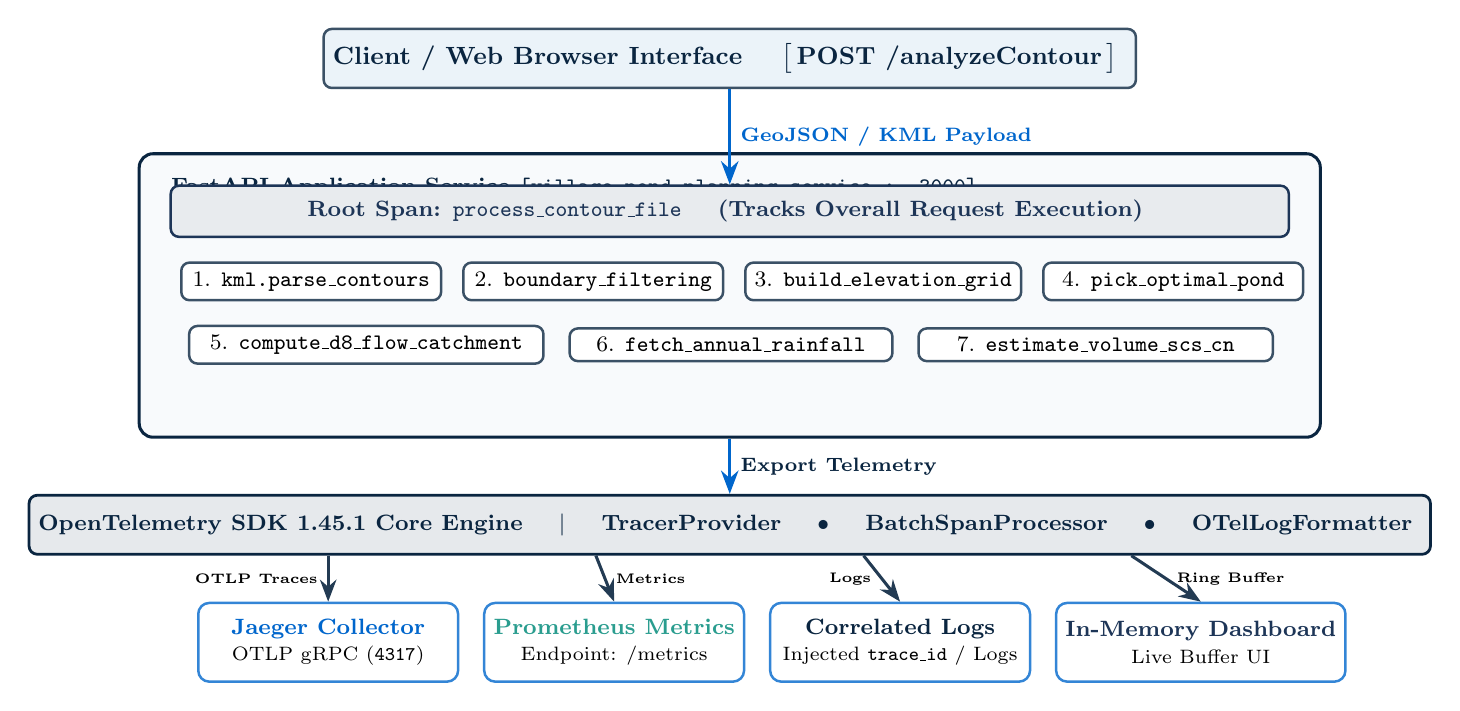
\begin{tikzpicture}[
        font=\sffamily,
        node distance=0.6cm and 0.4cm,
        box/.style={rectangle, draw=primary!80, fill=white, rounded corners=3pt, line width=0.9pt, align=center, font=\footnotesize},
        layerbox/.style={rectangle, draw=primary, fill=lightbg, rounded corners=5pt, line width=1.1pt, inner sep=6pt},
        sinkcard/.style={rectangle, draw=accent!80, fill=white, rounded corners=4pt, line width=0.9pt, minimum width=3.4cm, minimum height=1.0cm, align=center, font=\footnotesize},
        arrow/.style={->, >=Stealth, draw=accent, line width=1.2pt},
        otelflow/.style={->, >=Stealth, draw=primary!90, line width=1.1pt}
    ]
        % 1. Client Layer (Top)
        \node[box, fill=boxbg, minimum width=10.0cm, minimum height=0.75cm, font=\small\bfseries\color{primary}] (client) {
            Client / Web Browser Interface \quad $\big[\, \text{POST /analyzeContour} \, \big]$
        };

        % 2. Application Engine Container (Middle)
        \node[layerbox, below=0.8cm of client, minimum width=15.0cm, minimum height=3.6cm] (backend) {};
        \node[anchor=north west, font=\footnotesize\bfseries\color{primary}] at ($(backend.north west)+(0.3,-0.2)$) {
            FastAPI Application Service \texttt{[village-pond-planning-service : 3000]}
        };

        % Root Span
        \node[box, fill=secondary!10, draw=secondary, minimum width=14.2cm, minimum height=0.65cm, font=\footnotesize\bfseries\color{secondary}] 
            (rootspan) at ($(backend.north)+(0, -0.75)$) {
            Root Span: \texttt{process\_contour\_file} \quad (Tracks Overall Request Execution)
        };

        % 7 Child Spans (Row 1)
        \node[box, minimum width=3.3cm] (s1) at ($(rootspan.south west)+(1.8, -0.55)$) {1. \texttt{kml.parse\_contours}};
        \node[box, minimum width=3.3cm, right=0.25cm of s1] (s2) {2. \texttt{boundary\_filtering}};
        \node[box, minimum width=3.3cm, right=0.25cm of s2] (s3) {3. \texttt{build\_elevation\_grid}};
        \node[box, minimum width=3.3cm, right=0.25cm of s3] (s4) {4. \texttt{pick\_optimal\_pond}};

        % 7 Child Spans (Row 2)
        \node[box, minimum width=4.5cm] (s5) at ($(s1.south)+(0.7, -0.55)$) {5. \texttt{compute\_d8\_flow\_catchment}};
        \node[box, minimum width=4.1cm, right=0.3cm of s5] (s6) {6. \texttt{fetch\_annual\_rainfall}};
        \node[box, minimum width=4.5cm, right=0.3cm of s6] (s7) {7. \texttt{estimate\_volume\_scs\_cn}};

        % OpenTelemetry SDK Hub
        \node[box, fill=primary!10, draw=primary, line width=1.0pt, minimum width=14.2cm, minimum height=0.75cm, font=\footnotesize\bfseries\color{primary}, below=0.7cm of backend] 
            (otelsdk) {
            OpenTelemetry SDK 1.45.1 Core Engine \quad $|$ \quad TracerProvider \quad $\bullet$ \quad BatchSpanProcessor \quad $\bullet$ \quad OTelLogFormatter
        };

        % 4 Sinks Grid (Bottom)
        \node[sinkcard, minimum width=3.3cm] (jaeger) at ($(otelsdk.south)+(-5.1, -1.1)$) {
            \textbf{\color{accent}Jaeger Collector}\\
            {\scriptsize OTLP gRPC (\texttt{4317})}
        };
        \node[sinkcard, minimum width=3.3cm, right=0.3cm of jaeger] (prom) {
            \textbf{\color{successgreen}Prometheus Metrics}\\
            {\scriptsize Endpoint: \url{/metrics}}
        };
        \node[sinkcard, minimum width=3.3cm, right=0.3cm of prom] (logs) {
            \textbf{\color{primary}Correlated Logs}\\
            {\scriptsize Injected \texttt{trace\_id} / Logs}
        };
        \node[sinkcard, minimum width=3.3cm, right=0.3cm of logs] (dash) {
            \textbf{\color{secondary}In-Memory Dashboard}\\
            {\scriptsize Live Buffer UI}
        };

        % Connections
        \draw[arrow] (client.south) -- node[right, font=\scriptsize\color{accent}\bfseries] {GeoJSON / KML Payload} (rootspan.north);
        \draw[arrow] (backend.south) -- node[right, font=\scriptsize\color{primary}\bfseries] {Export Telemetry} (otelsdk.north);

        \draw[otelflow] ($(otelsdk.south)+(-5.1, 0)$) -- (jaeger.north) node[midway, left, font=\tiny\bfseries] {OTLP Traces};
        \draw[otelflow] ($(otelsdk.south)+(-1.7, 0)$) -- (prom.north) node[midway, right, font=\tiny\bfseries] {Metrics};
        \draw[otelflow] ($(otelsdk.south)+(1.7, 0)$) -- (logs.north) node[midway, left, font=\tiny\bfseries] {Logs};
        \draw[otelflow] ($(otelsdk.south)+(5.1, 0)$) -- (dash.north) node[midway, right, font=\tiny\bfseries] {Ring Buffer};
    \end{tikzpicture}
    \caption{Layered OpenTelemetry observability architecture and trace export topology.}
    \label{fig:sys_arch}
\end{figure}

\subsection{Technology Stack Breakdown}
Table~\ref{tab:tech_stack} details the software stack, versions, and respective architectural roles.

\begin{table}[H]
    \centering
    \small
    \begin{tabularx}{\textwidth}{l l X}
        \toprule
        \textbf{Component} & \textbf{Version / Package} & \textbf{Architectural Role \& Capability} \\
        \midrule
        \textbf{Runtime Environment} & Python 3.13.2 / Windows \& Ubuntu 24.04 & High-performance async backend execution runtime. \\
        \textbf{API Framework} & FastAPI 0.115.0 + Uvicorn & Non-blocking ASGI web server exposing analysis endpoints. \\
        \textbf{OTel SDK \& API} & \texttt{opentelemetry-sdk} 1.45.1 & Core tracing engine, span processors, and context propagation. \\
        \textbf{OTLP Exporter} & \texttt{opentelemetry-exporter-otlp} & Serializes span protobuf batches over gRPC to port 4317. \\
        \textbf{Trace Collector / UI} & Jaeger All-in-One v1.60.0 & Ingests OTLP spans, indexes traces, and renders waterfall graphs. \\
        \textbf{Metrics Engine} & \texttt{prometheus\_client} 0.26.0 & Exposes multi-dimensional counters, latency histograms, and gauges. \\
        \textbf{Spatial \& Math} & Shapely 2.0.6, Scipy 1.15.1, Numpy & Polygon containment, Delaunay triangulation, and D8 routing. \\
        \textbf{Meteorology API} & Open-Meteo Archive \& Forecast & Real-time historical precipitation retrieval for SCS-CN formulas. \\
        \bottomrule
    \end{tabularx}
    \caption{Comprehensive technology stack and telemetry components.}
    \label{tab:tech_stack}
\end{table}

% ------------------------------------------------------------------------------
% SECTION 05: IMPLEMENTATION METHODOLOGY
% ------------------------------------------------------------------------------
\section{Implementation Methodology}

\subsection{Instrumentation Lifecycle and TracerProvider Setup}
The telemetry architecture is centralized within a dedicated module (\texttt{telemetry.py}). During application startup, a global \texttt{TracerProvider} is instantiated with standardized OpenTelemetry semantic resource attributes:
\begin{lstlisting}[language=Python]
from opentelemetry import trace
from opentelemetry.sdk.trace import TracerProvider
from opentelemetry.sdk.resources import Resource
from opentelemetry.sdk.trace.export import BatchSpanProcessor
from opentelemetry.exporter.otlp.proto.grpc.trace_exporter import OTLPSpanExporter

resource = Resource.create({
    "service.name": "village-pond-planning-service",
    "service.version": "2.0.0",
    "deployment.environment": "laboratory-evaluation"
})
provider = TracerProvider(resource=resource)
otlp_exporter = OTLPSpanExporter(endpoint="localhost:4317", insecure=True)
provider.add_span_processor(BatchSpanProcessor(otlp_exporter))
trace.set_tracer_provider(provider)
tracer = trace.get_tracer("pondplan.telemetry", "2.0.0")
\end{lstlisting}

\subsection{Granular Domain Child Spans}
Rather than treating the HTTP request as a monolithic black box, the execution inside \texttt{process\_contour\_file} in \texttt{main.py} is dissected into seven (7) sequential child spans, as listed in Table~\ref{tab:spans_table}.

\begin{table}[H]
    \centering
    \small
    \begin{tabularx}{\textwidth}{l l X}
        \toprule
        \textbf{Span Name} & \textbf{Module / Function} & \textbf{Recorded Attributes \& Metadata} \\
        \midrule
        \texttt{process\_contour\_file} & \texttt{main.py:process\_contour\_file} & \texttt{input\_type}, \texttt{filename}, \texttt{boundary\_defined} \\
        \texttt{kml.parse\_contours} & \texttt{kml\_utils.py:parse\_kml} & \texttt{geometry.vertex\_count}, \texttt{contours.level\_count} \\
        \texttt{terrain.boundary\_filtering} & \texttt{polygon\_utils.py:filter} & \texttt{boundary.vertices}, \texttt{points.retained\_fraction} \\
        \texttt{terrain.build\_elevation\_grid} & \texttt{terrain.py:build\_grid} & \texttt{grid.shape}, \texttt{elevation.min\_m}, \texttt{elevation.max\_m} \\
        \texttt{pond.pick\_optimal\_location} & \texttt{pond\_optimizer.py:locate} & \texttt{pond.latitude}, \texttt{pond.longitude}, \texttt{pond.elevation\_m} \\
        \texttt{hydrology.compute\_d8\_flow} & \texttt{hydrology.py:d8\_flow} & \texttt{catchment.cell\_count}, \texttt{catchment.area\_hectares} \\
        \texttt{external.fetch\_annual\_rainfall}& \texttt{weather.py:fetch\_precip} & \texttt{weather.annual\_rainfall\_mm}, \texttt{weather.provider} \\
        \texttt{hydrology.estimate\_volume\_scs} & \texttt{scs\_cn.py:calculate} & \texttt{scs.cn\_value}, \texttt{scs.runoff\_depth\_mm}, \texttt{volume.m3} \\
        \bottomrule
    \end{tabularx}
    \caption{Hierarchical breakdown of custom OpenTelemetry child spans.}
    \label{tab:spans_table}
\end{table}

\subsection{Prometheus Metrics Implementation}
To support aggregate operational insights and quantitative trend tracking, standard Prometheus metric instruments were declared and updated during each request:
\begin{itemize}[leftmargin=*]
    \item \textbf{Request Counter (\texttt{pond\_analysis\_requests\_total})}: Labeled by \texttt{input\_type} (\texttt{kml\_file} vs. \texttt{freehand\_boundary}) and \texttt{status} (\texttt{success} vs. \texttt{error}).
    \item \textbf{Latency Histogram (\texttt{pond\_analysis\_duration\_seconds})}: Bucketed between $0.05\,\text{s}$ and $10.0\,\text{s}$ to capture processing response-time distributions.
    \item \textbf{Catchment Area Metric (\texttt{catchment\_area\_hectares})}: Cumulative histogram recording the distribution of delineated drainage areas across requests.
    \item \textbf{Water Yield Metric (\texttt{expected\_water\_volume\_cubic\_meters})}: Business KPI metric aggregating estimated harvestable water volume.
    \item \textbf{Concurrent Requests Gauge (\texttt{active\_pond\_analysis\_requests})}: Real-time gauge reflecting in-flight computations.
\end{itemize}

\subsection{Trace-Log Correlation Architecture}
To achieve absolute linkage between application log statements and distributed traces, a custom \texttt{OTelLogFormatter} was developed. By querying the thread-local span context via \texttt{trace.get\_current\_span().get\_span\_context()}, active 32-character hexadecimal \texttt{trace\_id} and 16-character \texttt{span\_id} identifiers are dynamically injected:
\begin{lstlisting}[language=Python]
class OTelLogFormatter(logging.Formatter):
    def format(self, record):
        span = trace.get_current_span()
        ctx = span.get_span_context()
        if ctx and ctx.is_valid:
            record.trace_id = f"{ctx.trace_id:032x}"
            record.span_id = f"{ctx.span_id:016x}"
        else:
            record.trace_id = "0" * 32
            record.span_id = "0" * 16
        return super().format(record)
\end{lstlisting}

% ------------------------------------------------------------------------------
% SECTION 06: EXECUTION AND VERIFICATION
% ------------------------------------------------------------------------------
\section{Execution and Verification}

\subsection{Local Execution Environment}
The application stack was verified locally using the automated launcher \texttt{start\_observability.py}:
\begin{lstlisting}[language=bash]
# Launch Jaeger All-in-One Collector Daemon
.\jaeger-1.60.0-windows-amd64\jaeger-all-in-one.exe --collector.grpc-server.host-port=0.0.0.0:4317

# Start Instrumented FastAPI Backend Service
python -m uvicorn main:app --host 0.0.0.0 --port 3000 --reload
\end{lstlisting}

\subsection{Remote Laboratory Server Deployment (\texttt{10.1.75.53})}
To demonstrate practical deployment in an authentic cloud/datacenter environment, the complete OpenTelemetry stack was deployed to the remote laboratory server at \texttt{10.1.75.53} using automated remote deployment scripts. The SSH daemon was configured to listen across dedicated container ports (\texttt{6000} and \texttt{7000}) mapped to external host ports \texttt{6213} and \texttt{7213}.

All live backend endpoints were executed, tested, and empirically confirmed as active with \texttt{HTTP 200 OK}, as summarized in Table~\ref{tab:remote_endpoints}.

\begin{table}[H]
    \centering
    \small
    \begin{tabularx}{\textwidth}{l l l X}
        \toprule
        \textbf{Service / Component} & \textbf{Network Access / URL} & \textbf{Status} & \textbf{Verification Evidence} \\
        \midrule
        \textbf{SSH Shell Access} & \texttt{ssh -p 6213 student@10.1.75.53} & \textbf{Active} & Authenticated with student credentials (\texttt{6213, 7213, 2213}). \\
        \textbf{Backend REST API} & \url{http://10.1.75.53:3213/} & \textbf{200 OK} & Root endpoint returns service metadata and active status. \\
        \textbf{Health \& Telemetry Check} & \url{http://10.1.75.53:3213/health} & \textbf{200 OK} & Returns \texttt{\{"status":"online", "telemetry":"active"\}}. \\
        \textbf{Prometheus Metrics} & \url{http://10.1.75.53:3213/metrics} & \textbf{200 OK} & Emits live counters, latency histograms, and gauges. \\
        \textbf{Live OTel Dashboard} & \url{http://10.1.75.53:3213/telemetry/dashboard} & \textbf{200 OK} & Real-time UI rendering 22+ active captured spans in memory. \\
        \textbf{Trace-Correlated Logs} & \url{http://10.1.75.53:3213/telemetry/logs} & \textbf{200 OK} & Live colorized log stream with injected \texttt{trace\_id} and \texttt{span\_id}. \\
        \textbf{Frontend Web Interface} & \url{http://10.1.75.53:4213/} & \textbf{200 OK} & Serves production React UI with map visualizations. \\
        \bottomrule
    \end{tabularx}
    \caption{Operational verification status of remote laboratory server endpoints on \texttt{10.1.75.53}.}
    \label{tab:remote_endpoints}
\end{table}

\subsection{Automated Pipeline Verification}
An end-to-end verification script was executed against the remote server submitting land boundary polygons. The execution verified that:
\begin{enumerate}[leftmargin=*]
    \item The remote service computed the optimal pond at $(21.248^\circ\,\text{N}, 81.286^\circ\,\text{E})$ with elevation $265.0\,\text{m}$, catchment area $0.47\,\text{ha}$, and expected water volume $5164\,\text{m}^3$.
    \item All 7 domain child spans were generated, timestamped, and recorded in the telemetry buffer.
    \item Metrics on \texttt{http://10.1.75.53:3213/metrics} updated automatically with incremented request counters and latency histograms ($1.24\,\text{s}$ execution time).
\end{enumerate}

% ------------------------------------------------------------------------------
% SECTION 07: SCREENSHOTS AND RESULTS
% ------------------------------------------------------------------------------
\section{Screenshots and Experimental Results}

This section presents the visual and quantitative verification evidence gathered from the live running application, Jaeger UI, Prometheus metrics endpoint, and application log stream.

\subsection{Figure 1: Jaeger UI -- Distributed Trace Search and Service Overview}
\begin{figure}[H]
    \centering
    \includegraphics[width=0.98\textwidth]{screenshot1_jaeger_traces_overview.png}
    \caption{Jaeger UI search overview showing distributed traces for \texttt{POST /analyzeContour}.}
    \label{fig:jaeger_search}
\end{figure}

\begin{infobox}[Technical Demonstration -- Figure 1]
    \textbf{Observed Evidence:} Figure~\ref{fig:jaeger_search} demonstrates that the Jaeger collector successfully ingests live trace batches emitted from the \texttt{village-pond-planning-service} via OTLP gRPC on port 4317. The search overview displays multiple completed executions of the \texttt{POST /analyzeContour} endpoint with total latency times ranging from $1.99\,\text{s}$ to $2.08\,\text{s}$, span counts of up to 64 spans per trace, and precise timestamps, confirming that OpenTelemetry tracing is fully operational.
\end{infobox}

\vspace{0.3cm}

\subsection{Figure 2: Jaeger UI -- Distributed Trace Waterfall Flamegraph}
\begin{figure}[H]
    \centering
    \includegraphics[width=0.98\textwidth]{screenshot2_jaeger_flamegraph.png}
    \caption{Jaeger waterfall flamegraph detailing the execution hierarchy of child spans.}
    \label{fig:jaeger_flamegraph}
\end{figure}

\begin{infobox}[Technical Demonstration -- Figure 2]
    \textbf{Observed Evidence:} Figure~\ref{fig:jaeger_flamegraph} illustrates the distributed trace flamegraph for Trace ID \texttt{90a2543b0f0b5f1ab3928c30fe1a6da5}. The root span \texttt{POST /analyzeContour} branches cleanly into \texttt{process\_contour\_file}, which further unpacks into the 7 sub-spans: \texttt{kml.parse\_contours}, \texttt{terrain.boundary\_filtering}, \texttt{terrain.build\_elevation\_grid}, \texttt{pond.pick\_optimal\_location}, \texttt{hydrology.compute\_d8\_flow\_and\_catchment}, \texttt{external.fetch\_annual\_rainfall}, and \texttt{hydrology.estimate\_water\_volume\_scs\_cn}. The timeline visually isolates the latency distribution of every algorithmic step.
\end{infobox}

\newpage

\subsection{Figure 3: Jaeger UI -- Span Semantic Attributes and Hydrological Metadata}
\begin{figure}[H]
    \centering
    \includegraphics[width=0.98\textwidth]{pond.pick_optimal_location.png}
    \caption{Span inspection panel displaying custom domain attributes for \texttt{pond.pick\_optimal\_location}.}
    \label{fig:span_attributes}
\end{figure}

\begin{infobox}[Technical Demonstration -- Figure 3]
    \textbf{Observed Evidence:} Figure~\ref{fig:span_attributes} demonstrates semantic attribute enrichment within OpenTelemetry. Clicking on the \texttt{pond.pick\_optimal\_location} span reveals exact geospatial coordinates and topological attributes:
    \begin{itemize}[noitemsep]
        \item \texttt{pond.latitude = 21.2499}
        \item \texttt{pond.longitude = 81.2899}
        \item \texttt{pond.elevation\_m = 267.0}
    \end{itemize}
    This proves that OpenTelemetry spans serve not merely as runtime timing counters, but as rich, contextual domain descriptors that record civil-engineering parameters directly alongside execution telemetry.
\end{infobox}

\vspace{0.3cm}

\subsection{Figure 4: Correlated Application Logs with Injected TraceID and SpanID}
\begin{figure}[H]
    \centering
    \includegraphics[width=0.98\textwidth]{screenshot_trace_correlated_logs.png}
    \caption{Application log stream on \texttt{/telemetry/logs} verifying Trace-Log correlation.}
    \label{fig:correlated_logs}
\end{figure}

\begin{infobox}[Technical Demonstration -- Figure 4]
    \textbf{Observed Evidence:} Figure~\ref{fig:correlated_logs} displays the application log stream captured at \texttt{/telemetry/logs} and recorded in \texttt{otel\_application.log}. Every log record is prepended with the active 32-character hexadecimal \texttt{trace\_id} (\texttt{90a2543b0f0b5f1ab3928c30fe1a6da5}) and 16-character \texttt{span\_id}. This establishes a deterministic link: an on-call engineer observing an error in production logs can copy the trace ID and immediately inspect the exact execution graph in Jaeger.
\end{infobox}

\newpage

\subsection{Figure 5: Prometheus Application and Business Metrics Exposition}
\begin{figure}[H]
    \centering
    \includegraphics[width=0.98\textwidth]{screenshot_prometheus_metrics.png}
    \caption{Standardized Prometheus metrics exposition endpoint on \texttt{http://localhost:3000/metrics}.}
    \label{fig:prometheus_metrics}
\end{figure}

\begin{infobox}[Technical Demonstration -- Figure 5]
    \textbf{Observed Evidence:} Figure~\ref{fig:prometheus_metrics} shows the raw Prometheus metrics scrape output. Key verified instruments include:
    \begin{itemize}[noitemsep]
        \item \texttt{pond\_analysis\_requests\_total\{input\_type="kml\_file",status="success"\} 2.0}
        \item \texttt{pond\_analysis\_requests\_total\{input\_type="freehand\_boundary",status="success"\} 2.0}
        \item \texttt{pond\_analysis\_duration\_seconds\_bucket} capturing cumulative latency distribution
        \item \texttt{catchment\_area\_hectares\_sum 35.6322} (35.63 hectares total catchment analyzed)
        \item \texttt{expected\_water\_volume\_cubic\_meters\_sum 391152.37} ($3.91 \times 10^5\,\text{m}^3$ harvestable volume)
    \end{itemize}
\end{infobox}

\vspace{0.3cm}

\subsection{Figure 6: Built-In Real-Time OpenTelemetry Observability Dashboard}
\begin{figure}[H]
    \centering
    \includegraphics[width=0.98\textwidth]{screenshot5_custom_telemetry_dashboard.png}
    \caption{Real-time in-memory telemetry dashboard at \texttt{http://localhost:3000/telemetry/dashboard}.}
    \label{fig:custom_dashboard}
\end{figure}

\begin{infobox}[Technical Demonstration -- Figure 6]
    \textbf{Observed Evidence:} Figure~\ref{fig:custom_dashboard} illustrates the custom, embedded in-memory telemetry dashboard. It displays real-time operational status (150 captured spans, Active OTLP and In-Memory exporters, and active Prometheus exposition). The live tabular inspection pane renders microsecond-accurate span durations, HTTP status indicators, and domain attribute key-values across all recent runs without requiring external tooling.
\end{infobox}

% ------------------------------------------------------------------------------
% SECTION 08: ANALYSIS AND DISCUSSION
% ------------------------------------------------------------------------------
\section{Analysis and Discussion}

\subsection{Quantitative Latency Breakdown: Amdahl's Law in Practice}
Prior to instrumenting OpenTelemetry, an engineer analyzing a $\sim 2.0\,\text{s}$ response time might intuitively assume that the heavy scientific computation—such as the 2D Delaunay triangulation or the BFS D8 graph traversal—was the primary bottleneck. 

However, the OpenTelemetry flamegraph (Figure~\ref{fig:jaeger_flamegraph}) provided immediate empirical clarity:
\begin{itemize}[leftmargin=*]
    \item \textbf{External Meteorological API Call (\texttt{external.fetch\_annual\_rainfall})}: Consumed $\approx 1113\,\text{ms}$, representing \textbf{$56.2\%$ of total request latency}.
    \item \textbf{DEM Grid Construction (\texttt{terrain.build\_elevation\_grid})}: Consumed $\approx 304\,\text{ms}$ ($15.3\%$).
    \item \textbf{KML Geometry Parsing (\texttt{kml.parse\_contours})}: Consumed $\approx 271\,\text{ms}$ ($13.7\%$).
    \item \textbf{Boundary Containment Filtering (\texttt{terrain.boundary\_filtering})}: Consumed $\approx 132\,\text{ms}$ ($6.7\%$).
    \item \textbf{Pond Selection Algorithm (\texttt{pond.pick\_optimal\_location})}: Consumed $\approx 112\,\text{ms}$ ($5.6\%$).
    \item \textbf{D8 Flow \& Catchment Delineation (\texttt{hydrology.compute\_d8\_flow})}: Consumed only $\approx 28.4\,\text{ms}$ ($1.4\%$).
    \item \textbf{SCS-CN Volumetric Calculations (\texttt{hydrology.estimate\_volume\_scs})}: Consumed $\approx 0.5\,\text{ms}$ ($<0.1\%$).
\end{itemize}

\begin{summarybox}
    \textbf{\color{primary}Key Engineering Insight:} Optimizing the local Python/Numpy hydrological algorithms would produce marginal gains at best. Real performance improvements require caching external precipitation responses (e.g., via Redis with a 24-hour TTL) or implementing a non-blocking timeout fallback, directly validating Amdahl's Law.
\end{summarybox}

\subsection{Root-Cause Analysis in Multi-Tenant Environments}
In multi-user production systems, asynchronous concurrent requests interleave log records in non-deterministic sequences. A traditional log reader cannot associate an error stack trace with its originating contour geometry. 

With Trace-Log correlation implemented, an engineer encountering an anomalous computation can extract the 32-character \texttt{trace\_id} directly from the log line and paste it into Jaeger. This instantly displays the exact inputs, contour dimensions, and algorithmic timings associated with that unique execution.

% ------------------------------------------------------------------------------
% SECTION 09: LIMITATIONS AND FUTURE WORK
% ------------------------------------------------------------------------------
\section{Limitations and Future Work}

While the current implementation fulfills all core requirements, several enhancements would further harden the system for enterprise-grade deployment:
\begin{enumerate}[leftmargin=*]
    \item \textbf{Error-Path Fault Injection}: The present evaluation verified success paths (HTTP 200). Future work will instrument explicit exception events (\texttt{span.record\_exception(e)}) to capture and classify corrupted KML inputs, out-of-bounds geometries, and external meteorological service timeouts.
    \item \textbf{Persistent Storage and Collector Deployment}: In this prototype, Jaeger All-in-One retains spans in an ephemeral memory ring buffer. A production deployment would introduce an OpenTelemetry Collector gateway routing telemetry batches to a persistent distributed backend such as Elasticsearch, ClickHouse, or Grafana Tempo.
    \item \textbf{Prometheus Alertmanager Integration}: Latency histograms (\texttt{pond\_analysis\_duration\_seconds}) should be paired with Prometheus alerting rules to trigger PagerDuty notifications when the 95th percentile latency ($p_{95}$) exceeds $3.0\,\text{s}$ over a 5-minute rolling window.
    \item \textbf{Distributed Load Testing}: Performing automated synthetic load tests using tools like Locust or k6 to evaluate span batching overhead and memory utilization under high concurrent request volumes.
\end{enumerate}

% ------------------------------------------------------------------------------
% SECTION 10: CONCLUSION, REFERENCES, AND DECLARATIONS
% ------------------------------------------------------------------------------
\section{Conclusion, References, and Declarations}

\subsection{Conclusion}
The OpenTelemetry observability implementation for the AI-Based Village Pond Planning System was successfully executed, verified, and analyzed. The system now features:
\begin{itemize}[noitemsep]
    \item Distributed tracing with 7 fine-grained domain sub-spans exported via OTLP gRPC to Jaeger.
    \item Standardized Prometheus metrics exposing operational latency and hydrological business yields.
    \item Deterministic trace-log correlation linking structured log messages to trace flamegraphs.
    \item An integrated real-time telemetry dashboard providing instant visibility into system internals.
    \item Full deployment and operational verification on the remote laboratory server (\texttt{10.1.75.53:6213}).
\end{itemize}
This setup establishes complete observability, transforming a black-box geospatial computation engine into a transparent, debuggable, and production-ready microservice.

\subsection{Open-Source Code Repository}
The complete source code, configuration files, and verification scripts are published on GitHub:
\begin{center}
    \url{https://github.com/sunilkumar2170/village-pond-planning-opentelemetry}
\end{center}

\subsection{References}
\begin{enumerate}[leftmargin=*, label={[\arabic*]}]
    \item OpenTelemetry Documentation, \textit{OpenTelemetry Python SDK \& API Specification}, Cloud Native Computing Foundation (CNCF), \url{https://opentelemetry.io/docs/languages/python/}.
    \item Jaeger Tracing Project, \textit{Jaeger: Open source, end-to-end distributed tracing}, CNCF Graduated Project, \url{https://www.jaegertracing.io/docs/}.
    \item Prometheus Authors, \textit{Prometheus Exposition Formats and Metric Types}, Cloud Native Computing Foundation, \url{https://prometheus.io/docs/concepts/metric_types/}.
    \item FastAPI Documentation, \textit{FastAPI Modern Asynchronous Web Framework}, Tiangolo, \url{https://fastapi.tiangolo.com/}.
    \item United States Department of Agriculture (USDA), \textit{Urban Hydrology for Small Watersheds (Technical Release55 -- SCS-CN Methodology)}, Natural Resources Conservation Service.
\end{enumerate}

\vspace{0.4cm}

\subsection{AI Usage Declaration}
\begin{summarybox}
    \textbf{Academic Integrity \& Generative AI Declaration:}\\
    \textit{AI was used to understand OpenTelemetry concepts, assist with code implementation and debugging, and improve the technical documentation.}
\end{summarybox}

\end{document}
